\documentclass[12pt]{article}

\usepackage[margin=1in]{geometry}
\usepackage{amssymb}
\usepackage{amsmath}
\usepackage{graphicx}
\usepackage{subcaption}
\usepackage{cleveref}       % this package must be loaded at the last

\setlength{\parskip}{1em}


\newenvironment{question}[2][Question]{\begin{trivlist}
\kern10pt
\item[\hskip \labelsep {\bfseries #1}\hskip \labelsep {\bfseries #2.}]}{\end{trivlist}}


\begin{document}

\title{DD2424 Deep Learning in Data Science Assignment 4}
\author{Lin Chun Hung, chlin3@kth.se}

\maketitle

\section{Basic Part (Part 1)}

\begin{question}{i}
I used the central difference method to calculate the numerical gradients
with respect to all the network parameters and used it check against with the
analytical gradients.

I checked the maximum relative error which was mentioned in assignment and I 
used the numpy function \texttt{numpy.testing.assert\_allclose} to test if 
the gradients calculated analytically and numerically are closed element-wise.
During this time, the RNN model was set to be calculated in double precision. 

For the maximum relative error, only the \texttt{grad\_output\_wgt} went up to 
0.033. I think it is okay as the numerical gradient is calculate after the non-linear
activation layer. Other gradient maximum relative errors are pretty low and 
which are expected.

For the test assertion, consider the following equation:
\begin{equation*}
    % absolute(a - b) <= (atol + rtol * absolute(b))
    |a - b| \leq (\texttt{atol} + \texttt{rtol} * |b|)
\end{equation*}
where \texttt{atol} and \texttt{rtol} are the tolerance parameters.
In the assertion, I set \texttt{atol} to be 1e-3 and \texttt{rtol} to be 1e-4.

With these checking, I considered my analytical gradient calculations were bug free.
\end{question}

\begin{question}{ii}
I ran the training for 10 epochs, the smooth function is plotted in 
\cref{plt:smooth_lost_basic_rnn}.

\begin{figure}[h]
    \centering
    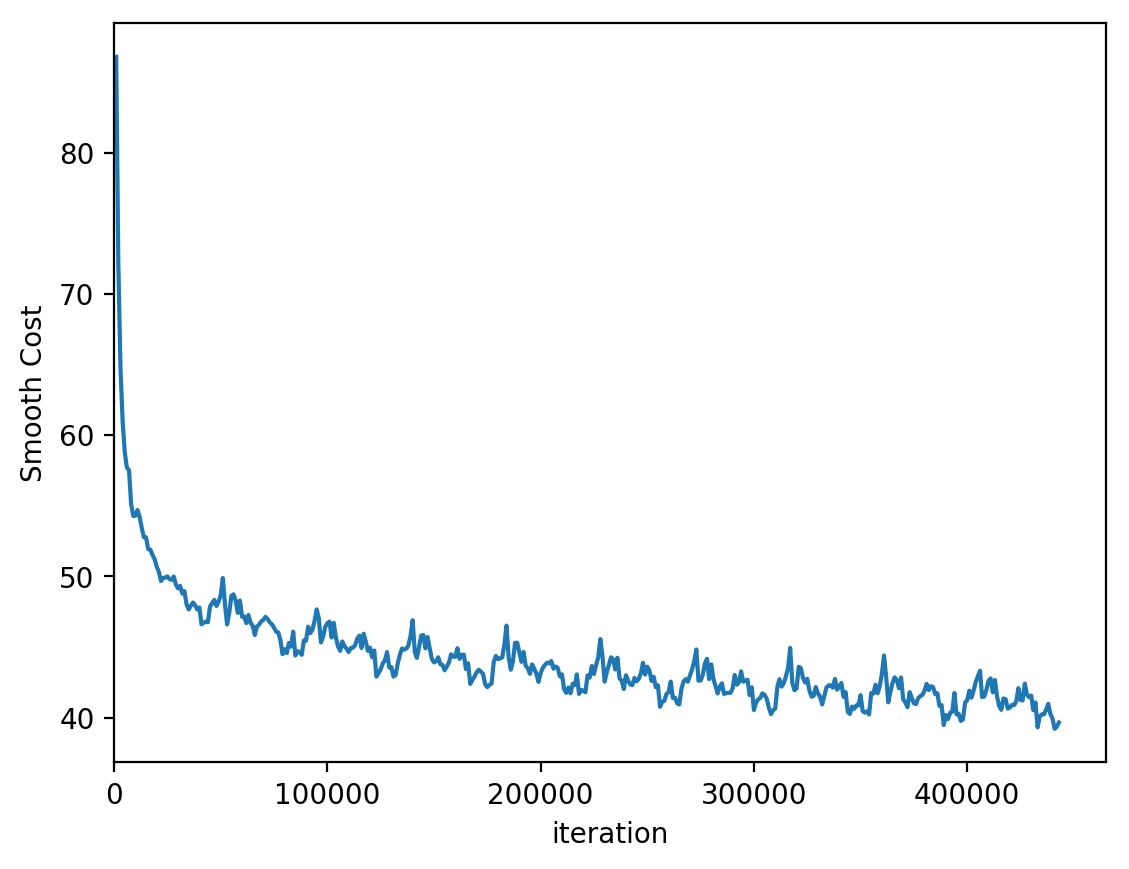
\includegraphics[width=0.8\textwidth]{./basic_cost.png}
    \caption{The smooth loss function plot}
    \label{plt:smooth_lost_basic_rnn}
\end{figure}
\end{question}

\begin{question}{iii}
The evolution of the text synthesized by the RNN:

\textbf{Iteration: 10000; smooth\_loss: 54.300842}

wadl't no oflen and Taroum sarr.  Arin ioBs tow?"
"Ave sbeks,e at cave yot lofm it wrat?"
Many, ckoary't no Slagkack, ds thamy Hurly, "Haulce to trom, wald riteraig Han. i coy.
"Goch bepny him she wav

\textbf{Iteration: 20000; smooth\_loss: 50.695659} 
Thar of thenenom in goor Rin piak beest mlemtiresease bicwing got at tle Doresjrofiro he to haillonked to bugance ald the lakK 'ilk, tor it inch Hiriaged, Kigon lecroke they rint and we ewaks'ch?"  bi

\textbf{Iteration: 30000; smooth\_loss: 49.151183} 
the groungerfirts was or the waider.  Harryd eee, was astid. . . baigagck in the reed over and of thoum!  Therimelnf.  Tall and hild.  "Harry . rars, sapkemas gevery prapur, as wis her sqommed firmirg

\textbf{Iteration: 40000; smooth\_loss: 47.801218} 
o wasce there Vortirn pawling od in thaigwan or and Harry.
"Vored; his werr tnew he iss foreracted and were in Vlasese'ld my cherered at with his his fundonarory him thing not eetrll was refave the tr

\end{question}

\end{document}
